\begin{frame}
\frametitle{About This Work...}

\emph{Graph Model Based Indoor Tracking}.~\cite{DBLP:conf/mdm/JensenLY09} \\
C.~S. Jensen, H.~Lu, and B.~Yang.\\~\\

\begin{itemize}
  \item Published in year 2009, \emph{MDM} conference.
  \item A pioneering work that introduces base graph model to indoor data management.
  \item Detailed tracking algorithms are designed for RFID-based positioning.
  \item Easy to understand, with comprehensive concepts.
\end{itemize}

\end{frame}

%------------------------------------------------

\begin{frame}
\frametitle{Motivation}

\begin{itemize}
  \item We are spending most of our time in indoor spaces
      \begin{itemize}
        \item Office building, University, Shopping Centers, etc.
      \end{itemize}
  \item We cannot use GPS-based tracking indoor movements
      \begin{itemize}
        \item Indoor navigation and route guidance (museum)
        \item Flow analysis
            \begin{itemize}
              \item how do people use the indoor space $\rightarrow$ important in pricing of advertisement space in store rental
            \end{itemize}
      \end{itemize}
  \item We can use other technology...
      \begin{itemize}
        \item Wi-Fi, Infrared, Bluetooth or RFID
        \item This paper is focusing on RFID, since it is now mature and effortless
        \item RFID tags are cheap and RFID reader are expensive
      \end{itemize}
\end{itemize}

\end{frame}

%------------------------------------------------

\begin{frame}
\frametitle{Idea}

\begin{columns}[c]

  \column{.6\textwidth}
    \begin{figure}[tb]
      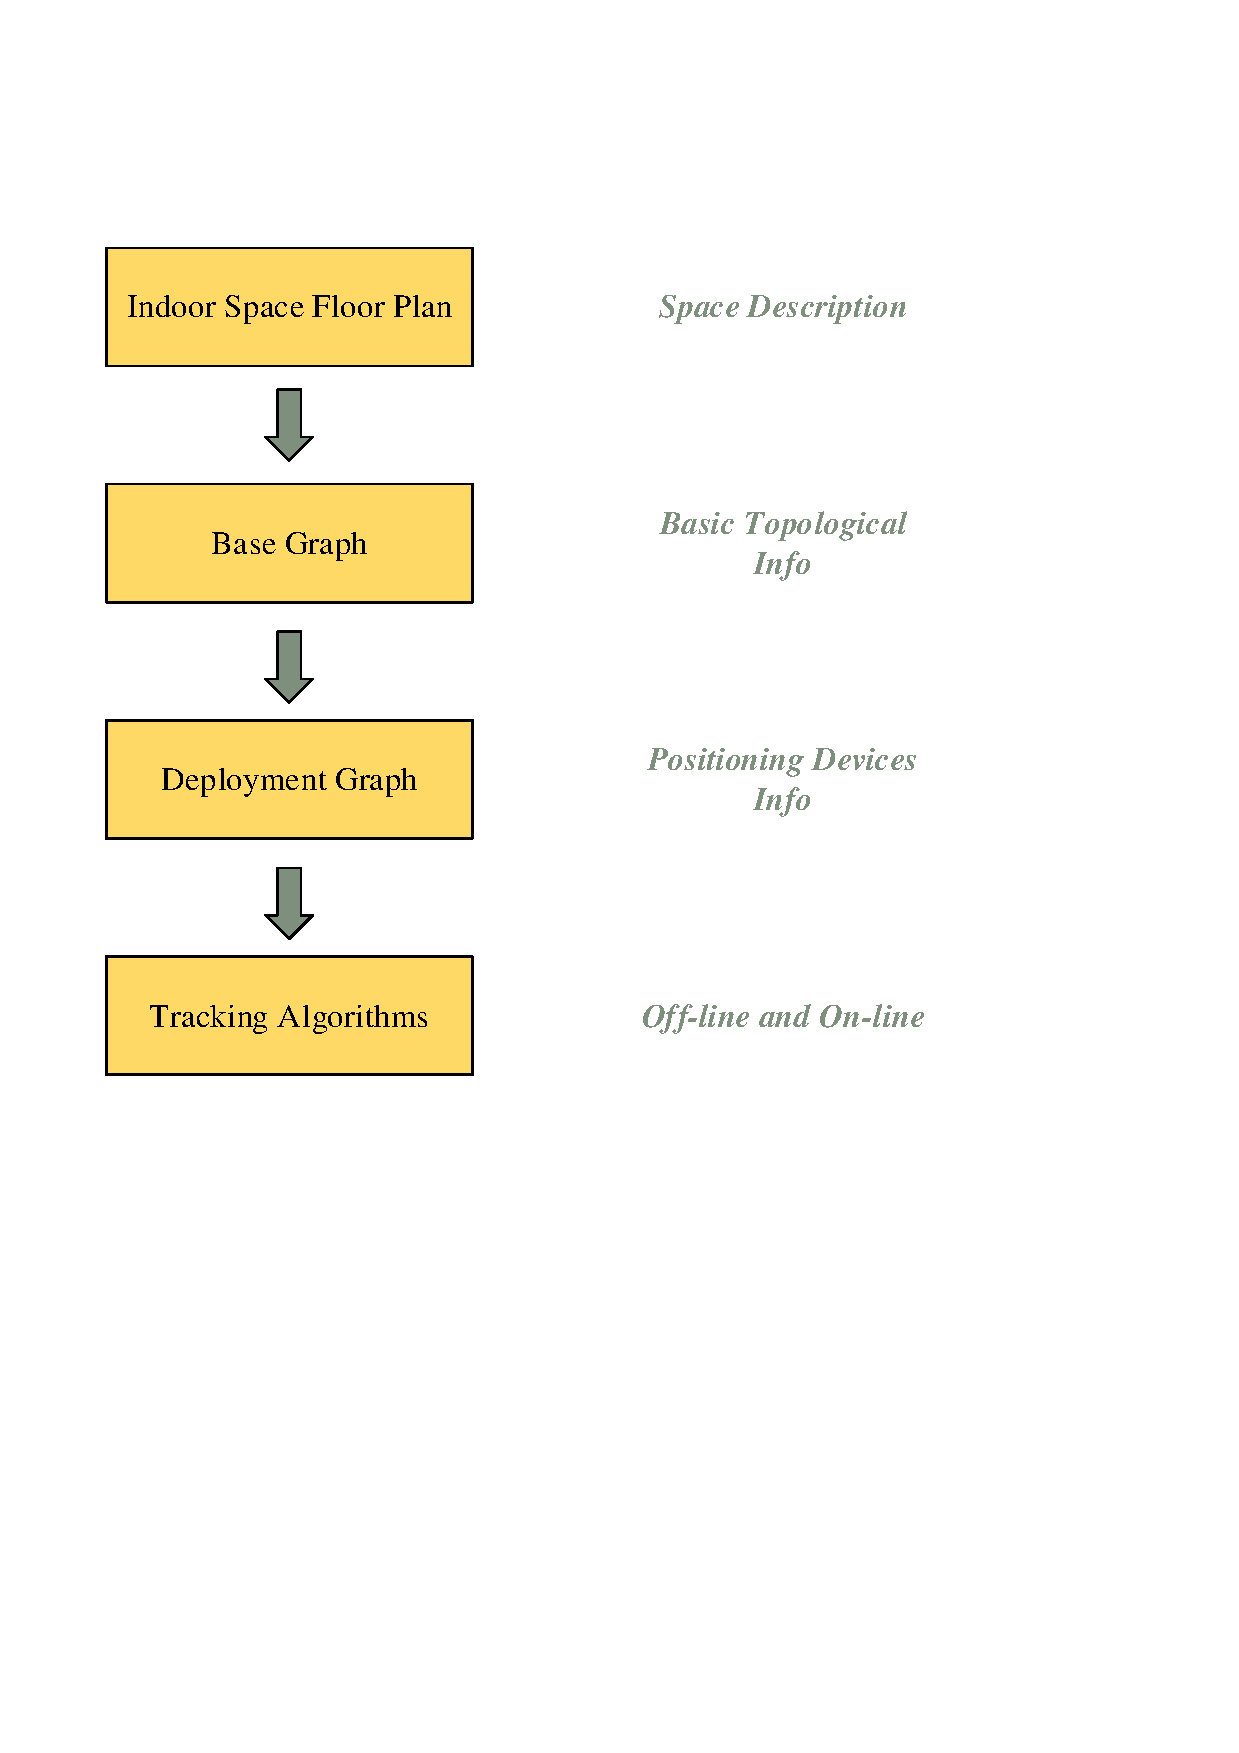
\includegraphics[width=\columnwidth]{figures/2-1-1.pdf}
    \end{figure}

  \column{.4\textwidth}
    \pause
    \textbf{Goal:} \textrm{Improve indoor tracking accuracy from a data management perspective, to capture where a particular object can be at a particular time.}

\end{columns}

\end{frame}

%------------------------------------------------

\begin{frame}
\frametitle{Base Graph Model}

\small{By capturing the essential connectivity and accessibility, \textbf{Base Graph} describes the topology of a floor plan of a possibly complex indoor space.}

\begin{columns}[c]

  \column{.45\textwidth}
    \begin{figure}[tb]
      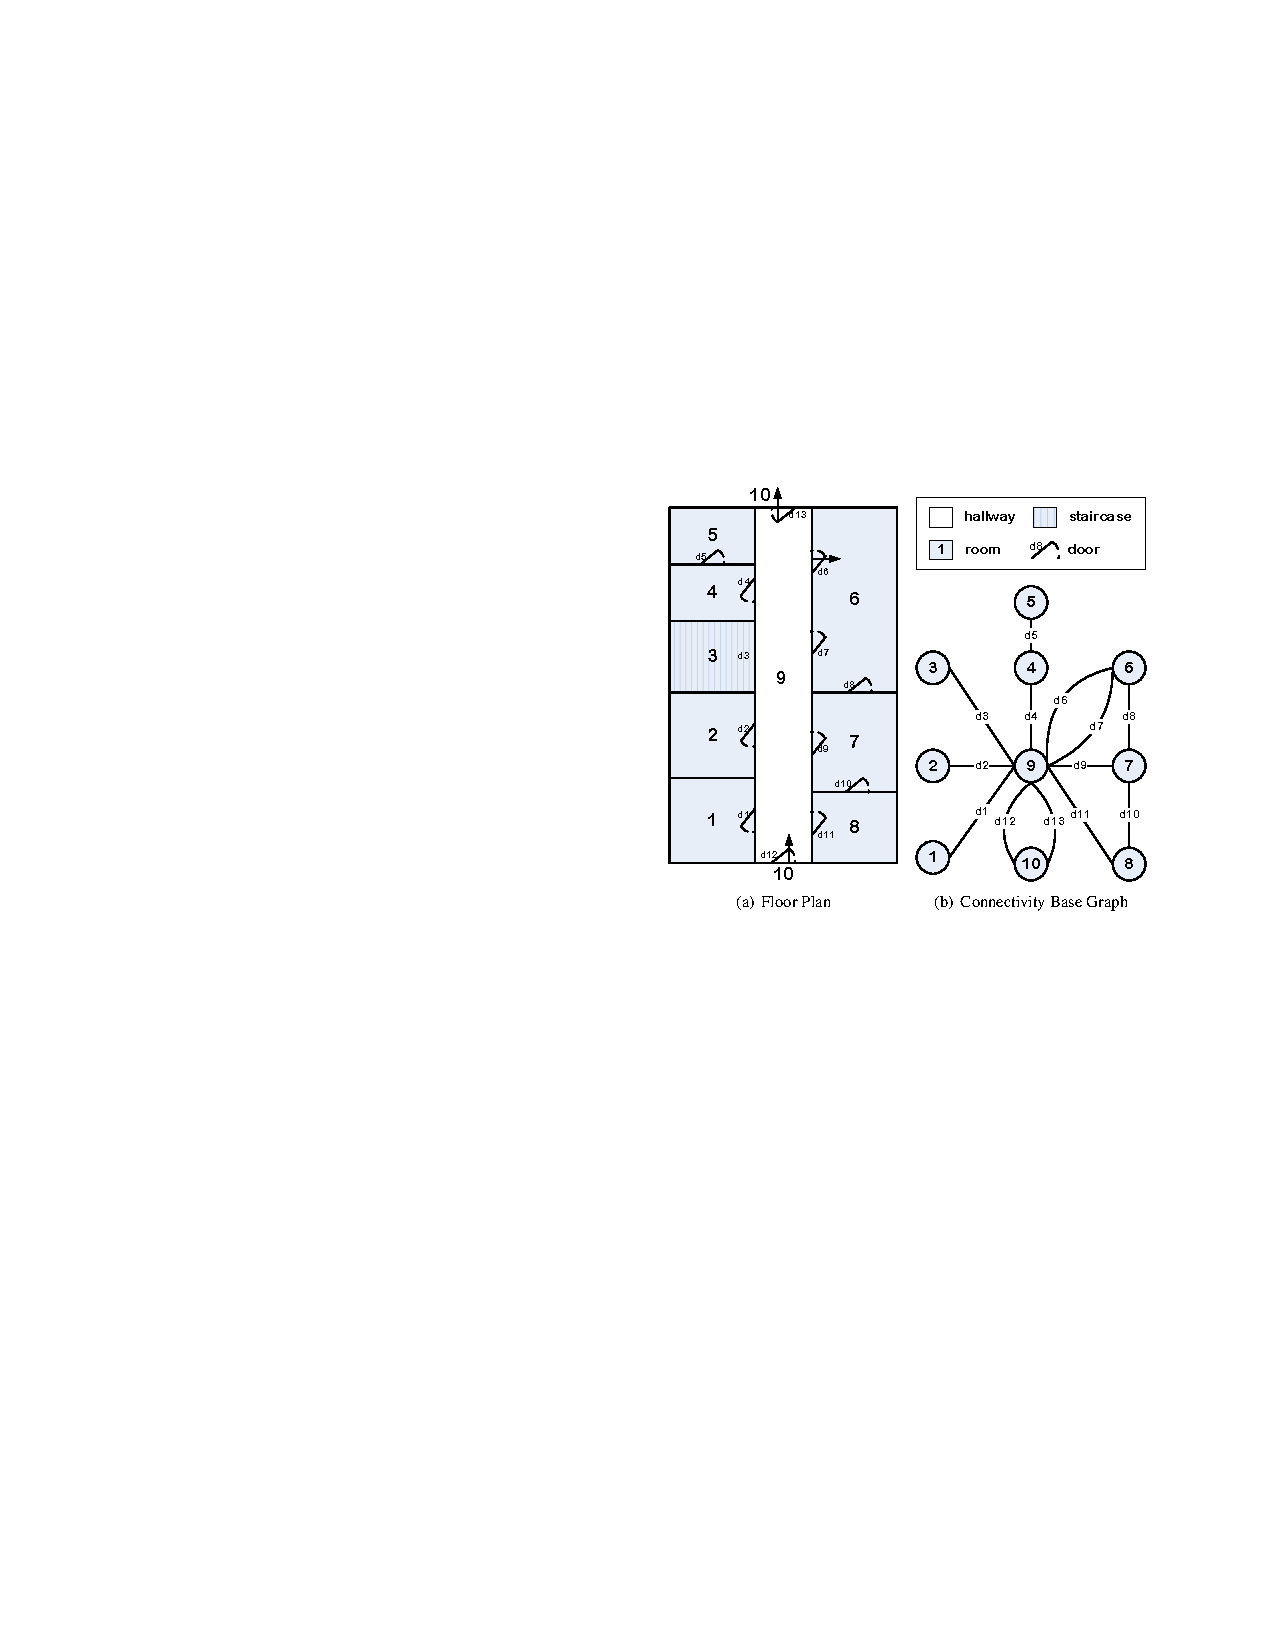
\includegraphics[width=\columnwidth]{figures/2-1-2.pdf}
    \end{figure}

  \column{.55\textwidth}
    \begin{block}{Connectivity Base Graph}
    a labeled, undirected graph.
      \textrm{
      \begin{itemize}
        \item $\mathnormal{G_{conn} = \{V, E_d, \Sigma_{door}\}}$
        \item $\mathnormal{V}$: each separate partition is represented as a vertex
        \item $\mathnormal{E_d}$: each door is captured as an edge%, i.e., $\mathnormal{(\{v_i,v_j}, k)}$
        \item $\mathnormal{\Sigma_{door}}$: a set of edge labels that represent connections
      \end{itemize}
      }
    \end{block}

\end{columns}
\end{frame}

%------------------------------------------------

\begin{frame}
\frametitle{Base Graph Model}

  \small{\textbf{Accessibility Graph} is constructed to represent the movement permitted by doors or connections.}

\begin{columns}[c]

  \column{.45\textwidth}
    \begin{figure}[tb]
      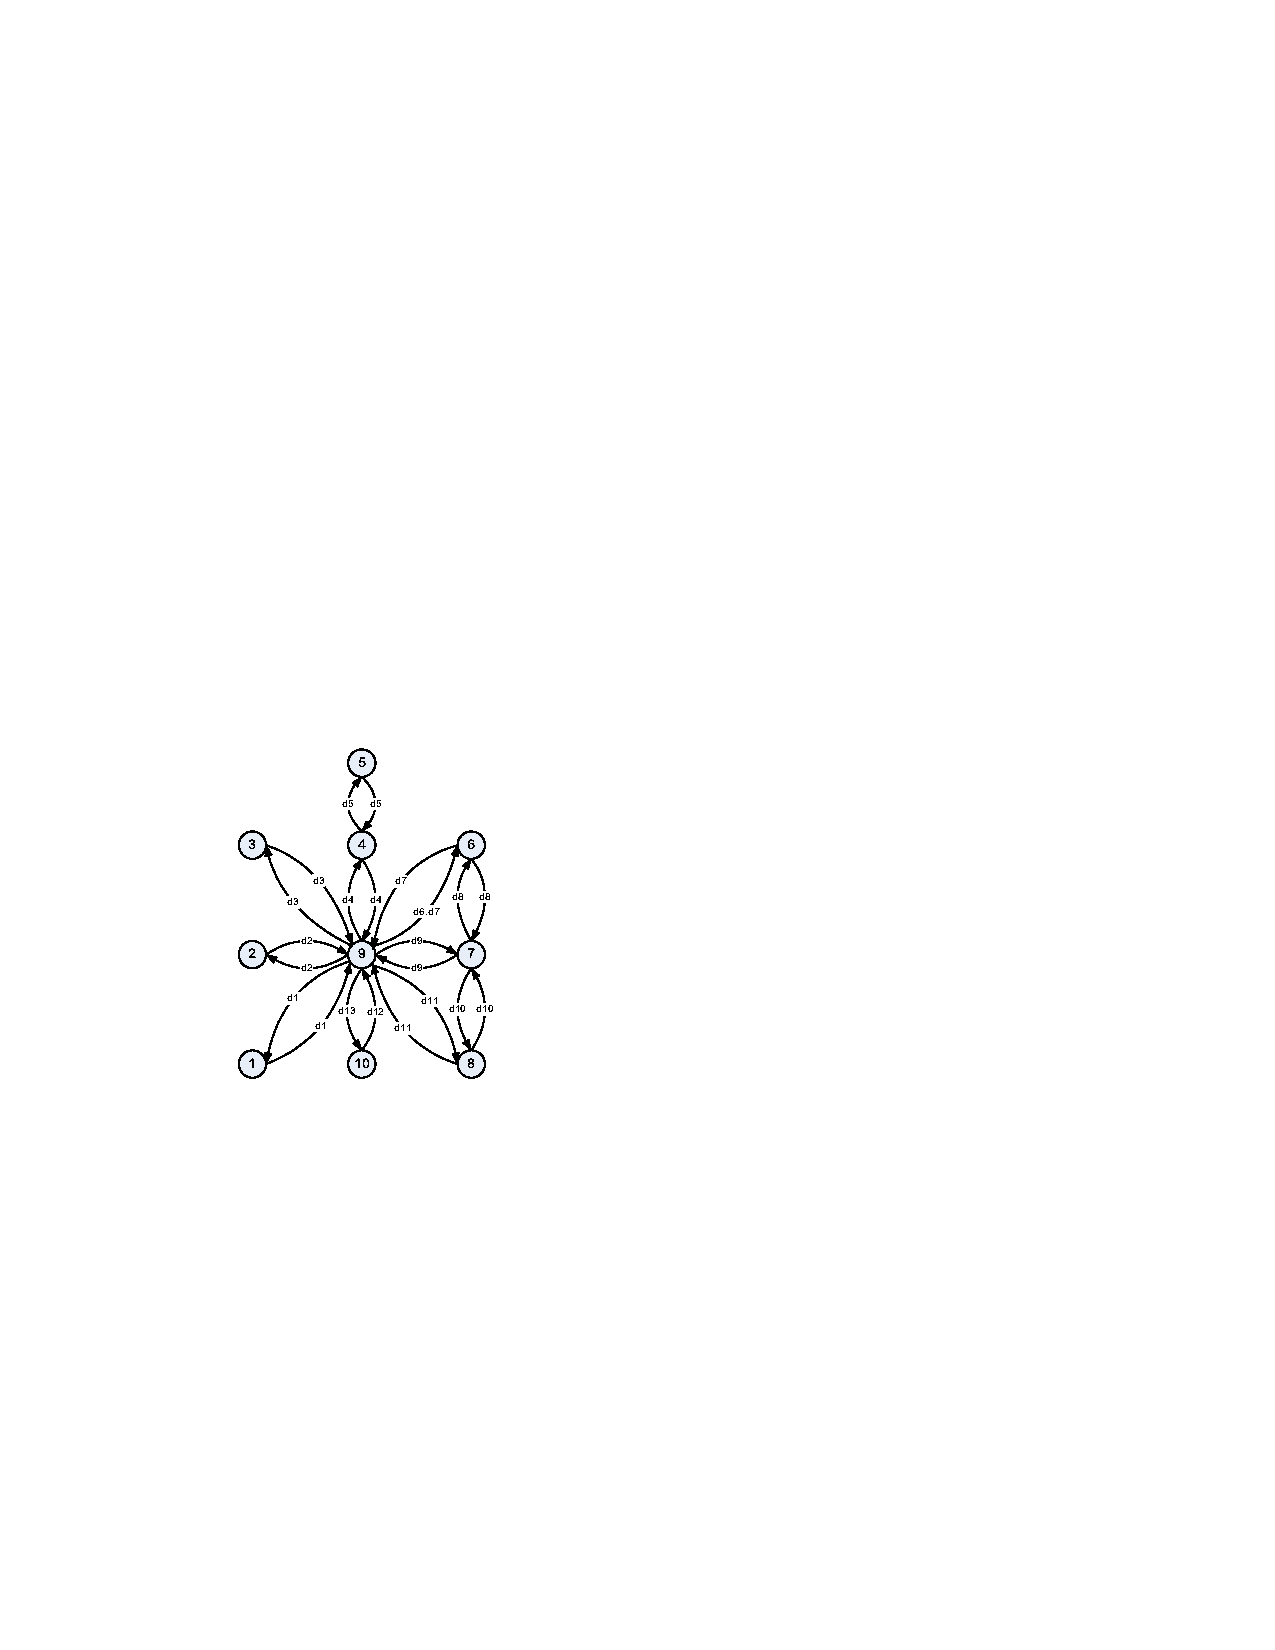
\includegraphics[width=\columnwidth]{figures/2-1-3.pdf}
    \end{figure}

  \column{.55\textwidth}
    \begin{block}{Accessibility Graph}
    a labeled, directed graph.
      \textrm{
      \begin{itemize}
        \item $\mathnormal{G_{accs} = \{V, E, \Sigma_{door}, l_e\}}$
        \item $\mathnormal{V}$: the set of vertices
        \item $\mathnormal{E}$: the set of directed edges, i.e., $\mathnormal{E=\{\langle v_i, v_j\rangle | v_i, v_j \in V \wedge v_i \neq v_j\}}$
        \item $\mathnormal{l_e}$: a function that maps edges to subsets of the set of doors, i.e., $\mathnormal{l_e : E \rightarrow 2^{\Sigma_{door}}}$
      \end{itemize}
      }
    \end{block}

\end{columns}
\end{frame}

%------------------------------------------------

\begin{frame}
\frametitle{Base Graph Model}

  \small{In addition to the topological information of a floor plan, its geometrical information should also be captured.}
  \\~\\
  \pause

  The \textrm{\em Building Partitions Mapping} is defined as:
  \pause
  \begin{equation}
  \mathnormal{BuildingPartitions: V \rightarrow Ploygons}
  \end{equation}
  \\~\\
  \pause

  The \textrm{\em Doors Mapping} is defined as:
  \pause
  \begin{equation}
  \mathnormal{Doors: \Sigma_{door} \rightarrow Line~Segments}
  \end{equation}

\end{frame}

%------------------------------------------------


\begin{frame}
\frametitle{RFID Deployment Graph Model}

\begin{itemize}
  \item RFID based proximity analysis
      \begin{itemize}
        %\item a record is produced when a \emph{RFID tag} approaches a \emph{RFID reader}.
        \item RFID readers deployment may cover only part of the space, or it may be capable of only detecting some movements in the space.
        \item assume that all RFID readers have disjoint activation ranges.
      \end{itemize}
  \item Types of RFID readers
      \begin{itemize}
        \item \textbf{Partitioning Readers} partition the indoor space into cells in the sense that an object cannot move from one cell to another without being observed.
        \item \textbf{Presence Readers} simply observe the presence(and non-presence) of tags in their activation ranges.
      \end{itemize}
\end{itemize}

\end{frame}

%------------------------------------------------

\begin{frame}
\frametitle{RFID Deployment Graph Model}

\small{Vertices represent cells. A directed edge indicates that one can move from one cell to another without entering other cells, which is detected by a corresponding partitioning reader.}

\begin{columns}[c]

  \column{.45\textwidth}
    \begin{figure}[tb]
      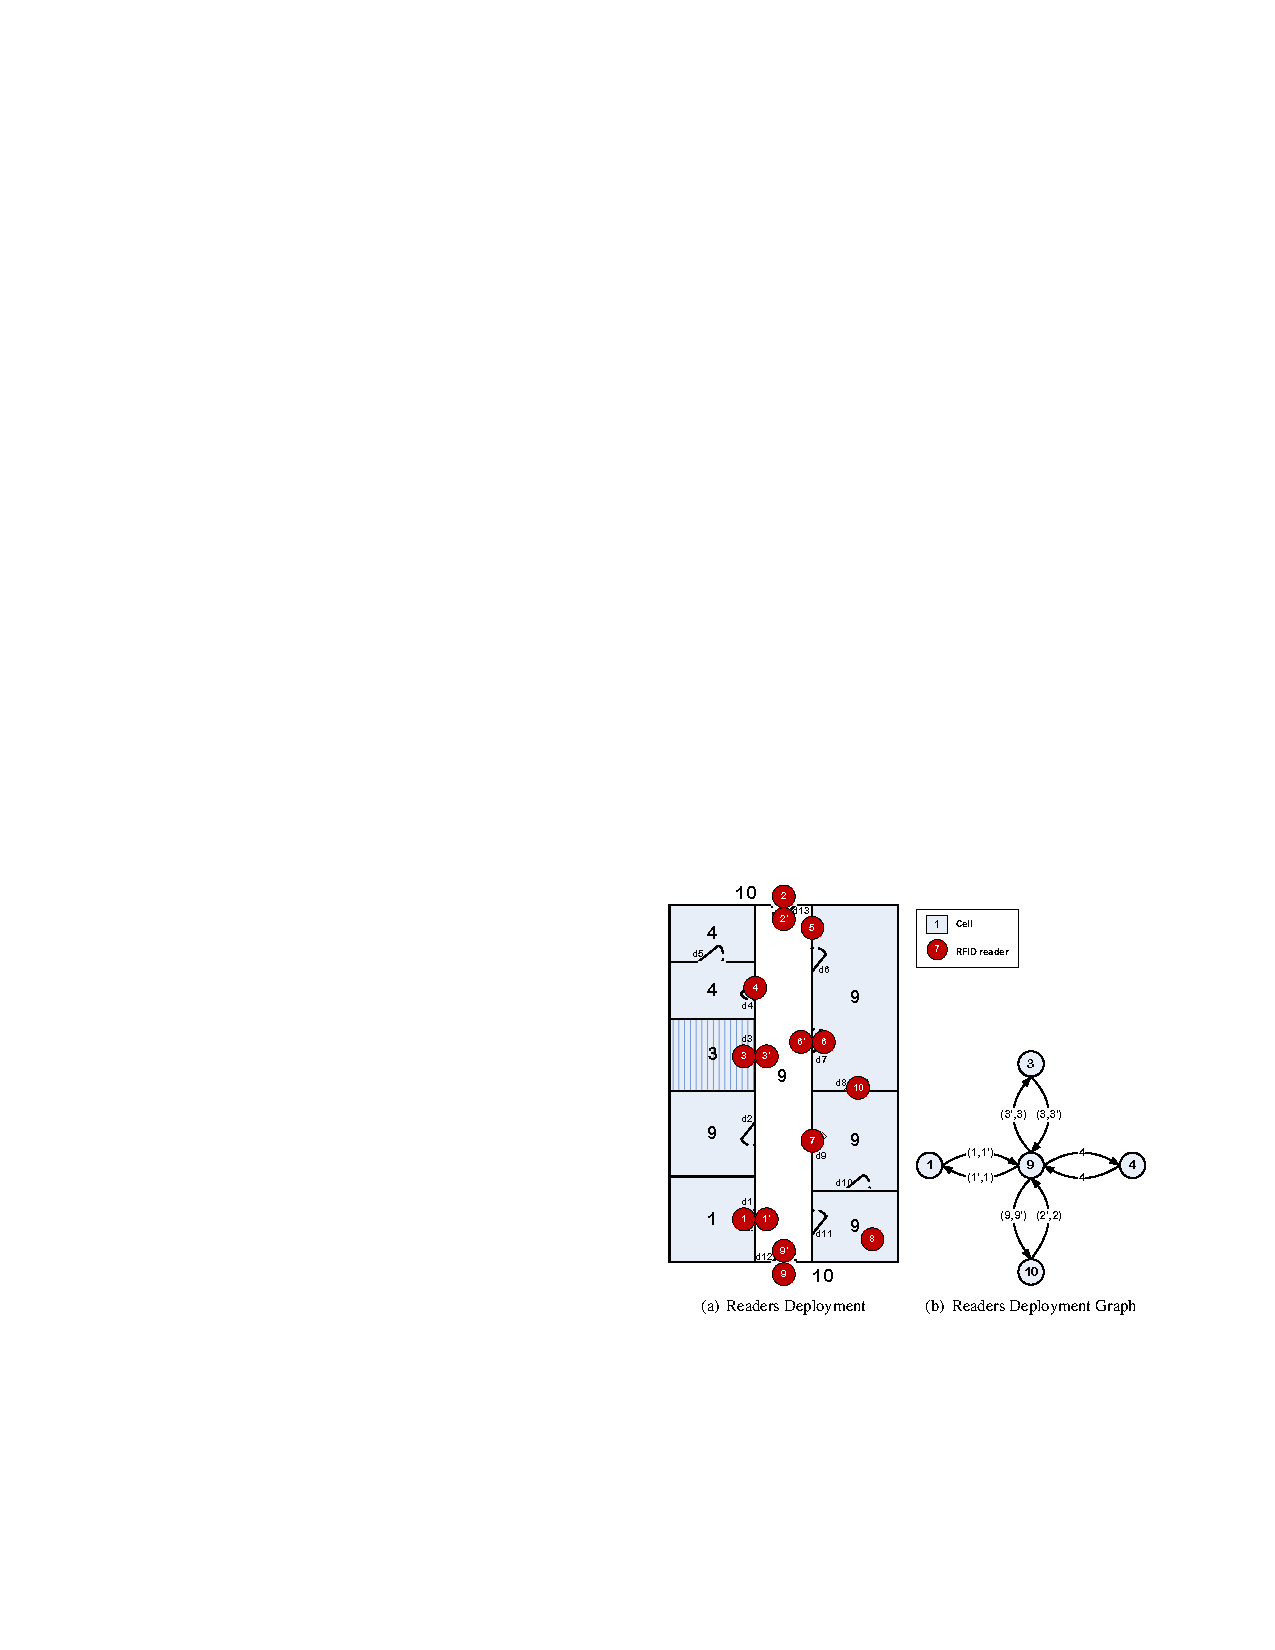
\includegraphics[width=\columnwidth]{figures/2-1-4.pdf}
    \end{figure}

  \column{.55\textwidth}
    \begin{block}{RFID Deployment Graph}
    a labeled, directed graph.
      \textrm{
      \begin{itemize}
        \item $\mathnormal{G_{RFID} = \{C, E_r, \Sigma_{reader}, l_e\}}$
        \item $\mathnormal{C}$: the set of the vertices
        \item $\mathnormal{E_r}$: An edge is an ordered pair $\mathnormal{\langle c_i, c_j \rangle}$ of distinct vertices from $\mathnormal{C}$
        \item $\mathnormal{l_e}$ maps an edge to a partitioning reader (pair), i.e., $\mathnormal{E_r \rightarrow 2^{\Sigma_{reader}} \cup 2^{\Sigma_{reader} \times \Sigma_{reader}}}$
      \end{itemize}
      }
    \end{block}

\end{columns}
\end{frame}

%------------------------------------------------

\begin{frame}
\frametitle{RFID Deployment Graph Construction}

  \small{Each cell created by partitioning readers corresponds to one or more base graph partitions.}
  \pause
  \begin{equation}
  \mathnormal{Cells: V \rightarrow C}
  \end{equation}
  \\~\\
  \pause

  \small{For each RFID reader, record its accurate deployment location and activation range.}
  \pause
  \begin{equation}
  \begin{split}
  \mathnormal{Mapping~1}: & \mathnormal{\Sigma_{reader} \rightarrow \{ (loc, range, flag)~|~loc \in R^2 \wedge} \\
    & \mathnormal{range \in (0,d_{max}] \wedge flag \in \{ PAR, PRE \} \}}
  \end{split}
  \end{equation}
  \\~\\
  \pause

  \small{A mapping of readers to the cells that their activation ranges intersect is introduced as:}
  \pause
  \begin{equation}
  \mathnormal{
  Mapping~2: \Sigma_{reader} \rightarrow 2^C
  }
  \end{equation}

\end{frame}

%------------------------------------------------

\begin{frame}
\frametitle{RFID Deployment Graph Construction}

\begin{columns}[c]

  \column{.47\textwidth}
    \begin{figure}[tb]
      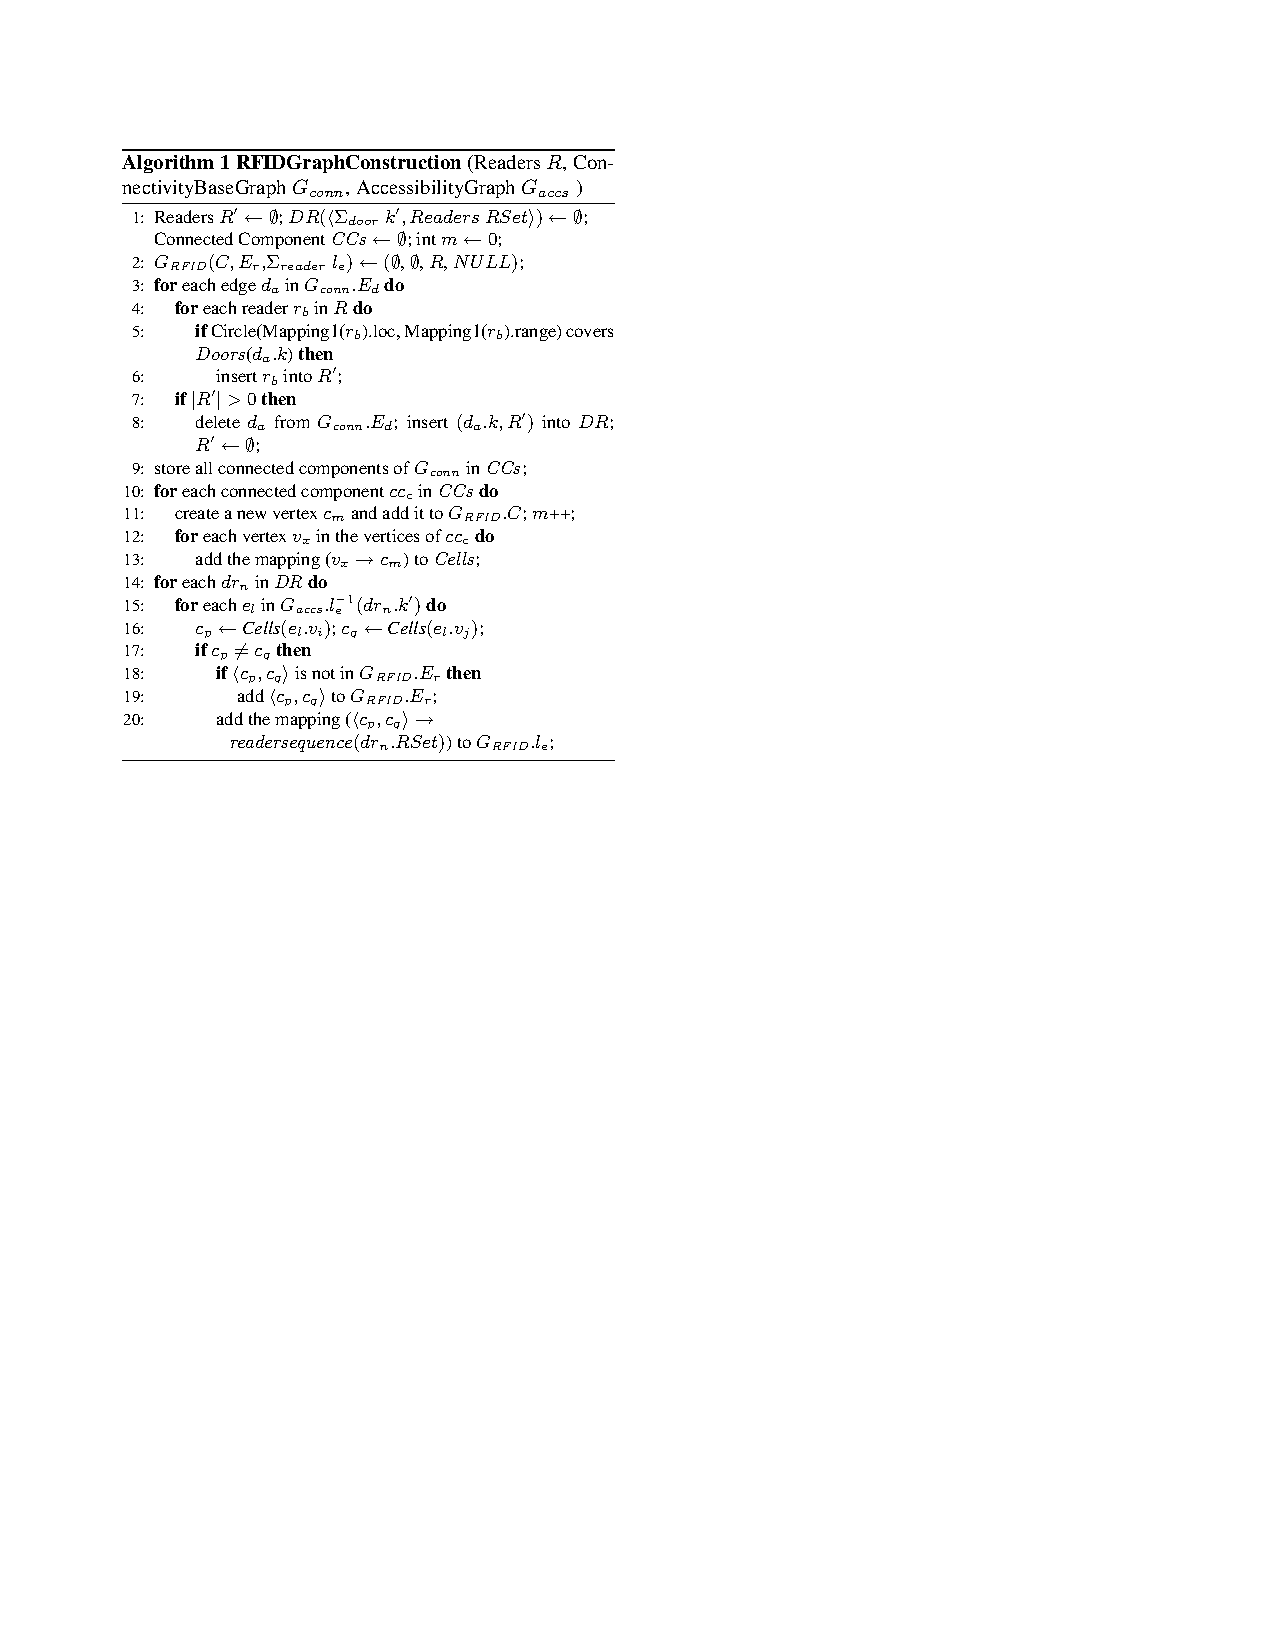
\includegraphics[width=\columnwidth]{figures/2-1-5.pdf}
    \end{figure}

  \column{.53\textwidth}
  \scriptsize{
    \begin{enumerate}
      \item Input: \textrm{the reader set $\mathnormal{R}$, the connectivity base graph $\mathnormal{G_{conn}}$, the accessibility graph $\mathnormal{G_{accs}}$} \pause
      \item Lines 1--2: \textrm{Initialize $\mathnormal{G_{RFID}}$, $\mathnormal{DR}$, $\mathnormal{CCs}$} \pause
      \item Lines 3--8: \textrm{the relationship of which door is covered by which readers is captured in $\mathnormal{DR}$} \pause
      \item Lines 9--13: \textrm{a deployment graph vertex is created for each $\mathnormal{CC}$, mapping $\mathnormal{Cells}$ is also stored} \pause
      \item Lines 14--20: \textrm{for each door in $\mathnormal{DR}$, determine if its edges' head and tail are mapped to different cells. If so, add an edge to deployment graph. Function $\mathnormal{readersequence}$ returns the possible reader sequence for that edge}
    \end{enumerate}
  }
  \end{columns}

\end{frame}

%------------------------------------------------

\begin{frame}
\frametitle{RFID-based Indoor Tracking}

  \small{\textbf{Raw Trajectories}: \textrm{Sequences of RFID Tag Observation}}

  \begin{columns}[c]

  \column{.47\textwidth}
    \begin{figure}[tb]
      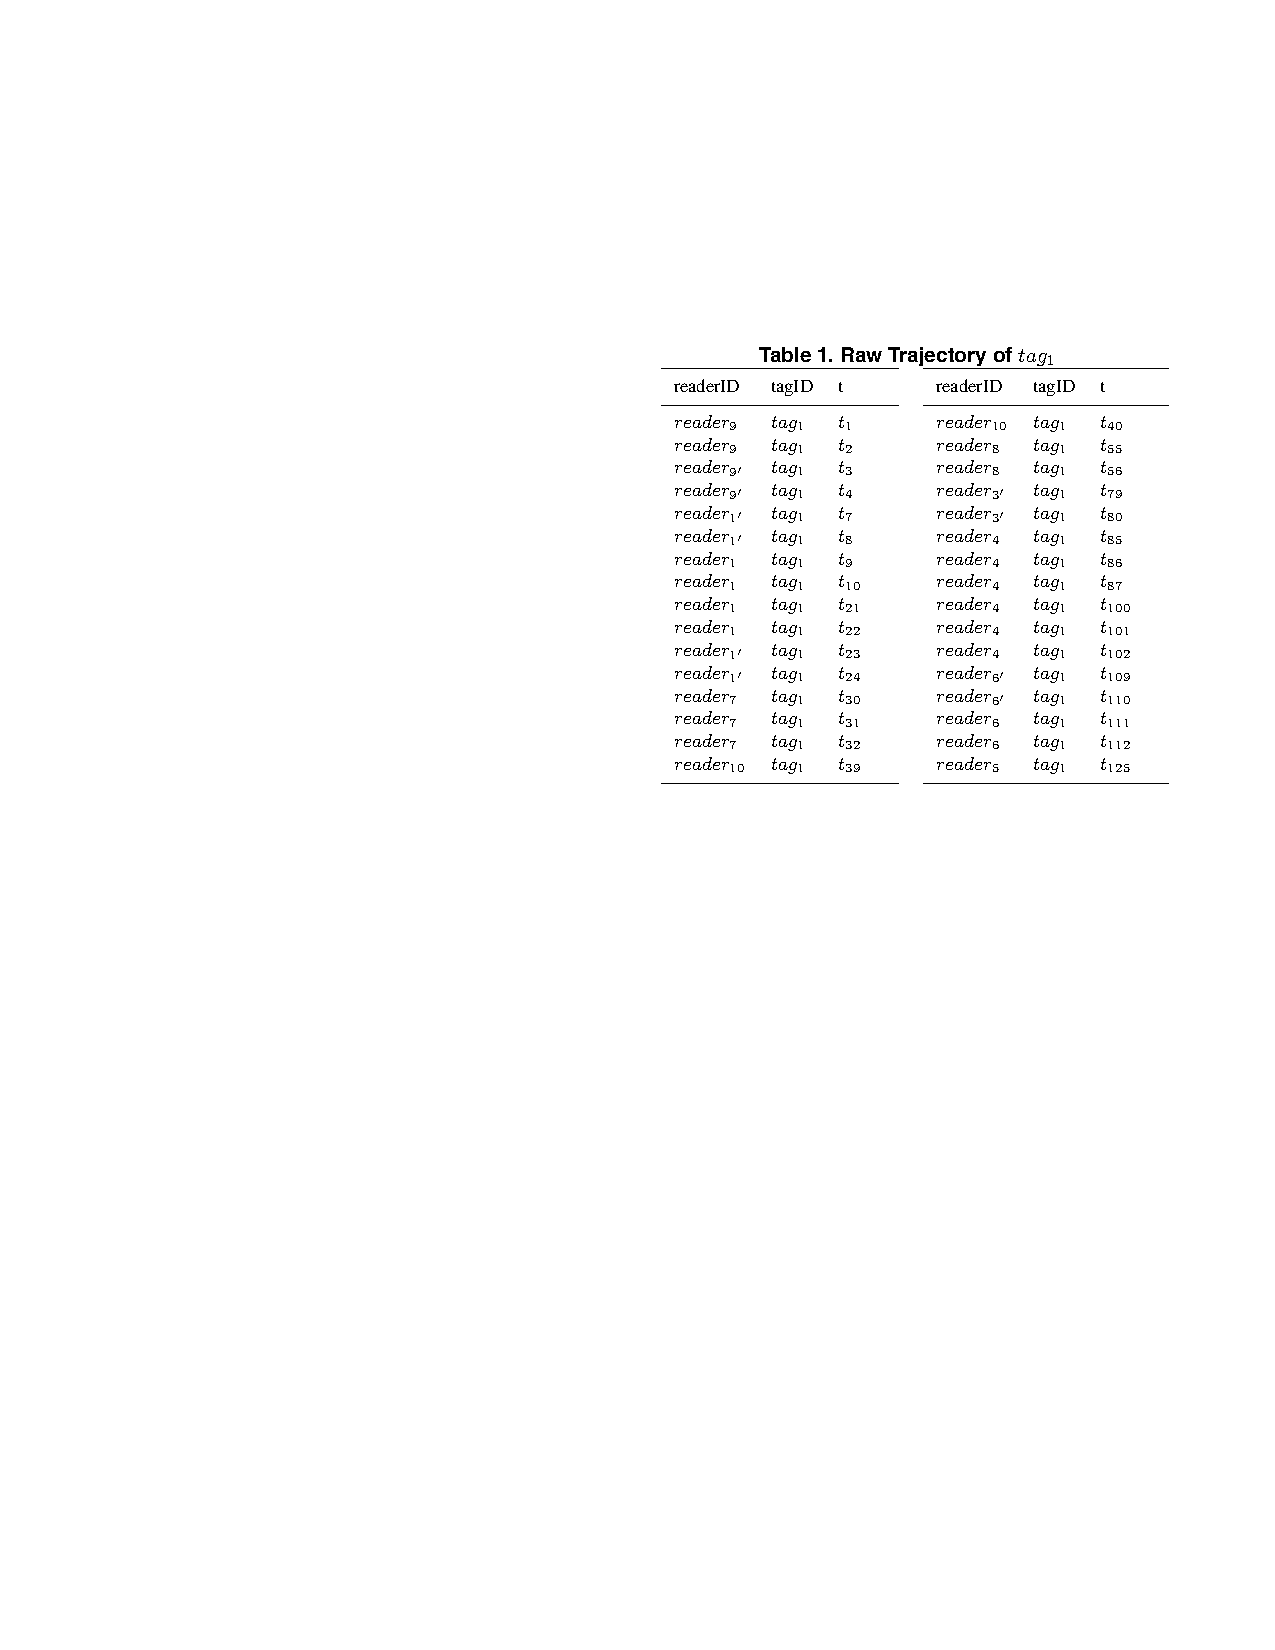
\includegraphics[width=\columnwidth]{figures/2-1-6.pdf}
    \end{figure}
    \scriptsize\textit{
      1. each reader detects and reports tags with a sampling rate \\
      2. formatted as $\mathnormal{\langle readerID, tagID, t \rangle}$
    }

  \column{.53\textwidth}
    \begin{figure}[tb]
      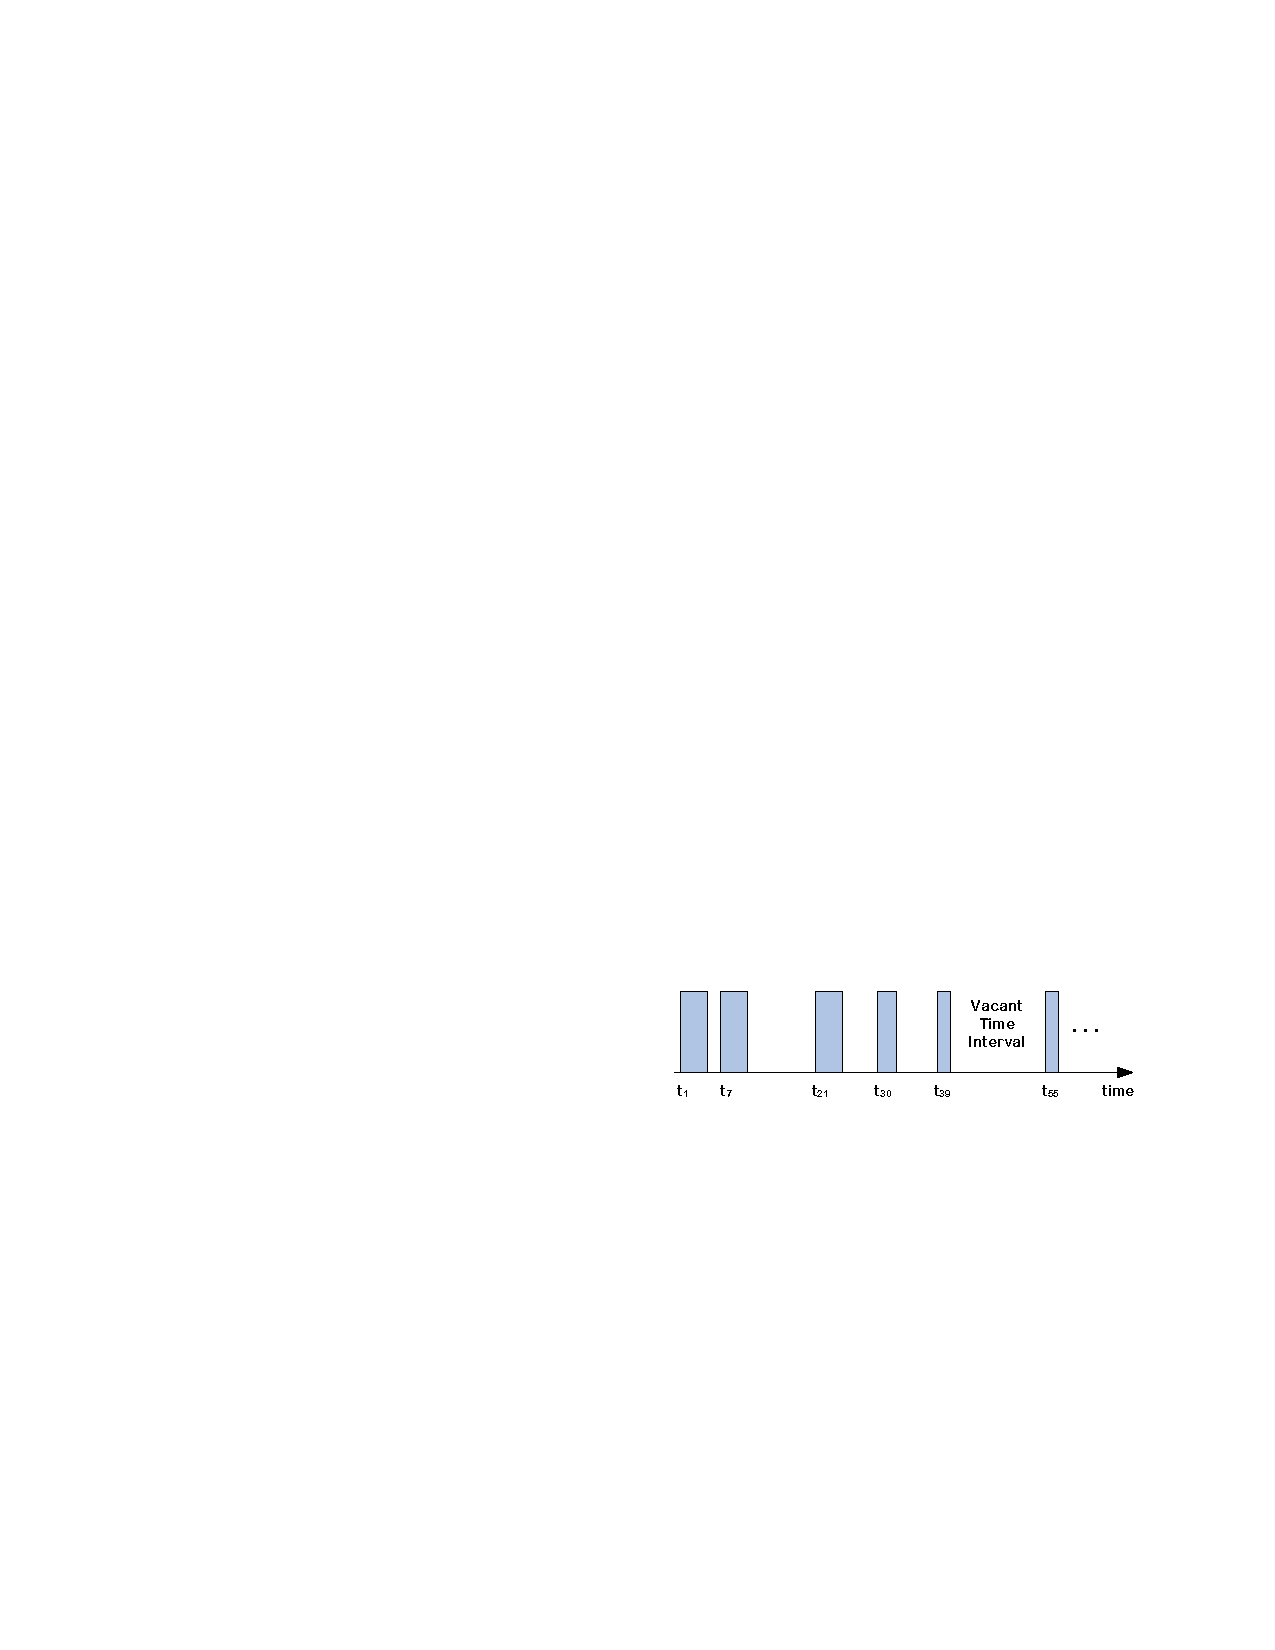
\includegraphics[width=\columnwidth]{figures/2-1-7.pdf}
    \end{figure}

    \vspace{-15pt}
    \scriptsize{
      \begin{itemize}
        \item \emph{vacant time intervals}: unable to observe the moving objects \pause
        \item to search RFID deployment graph to infer the possible regions of moving object \pause
        \item to apply maximum speed position interpolation to further shrink the possible regions
      \end{itemize}
    }

  \end{columns}

\end{frame}

%------------------------------------------------

\begin{frame}
\frametitle{RFID Readings Pre-processing}

  \small{Step-1's output is used in on-line tracking, while Step-2's is used in off-line tracking}

  \begin{columns}[c]

  \column{.47\textwidth}
    \begin{figure}[tb]
      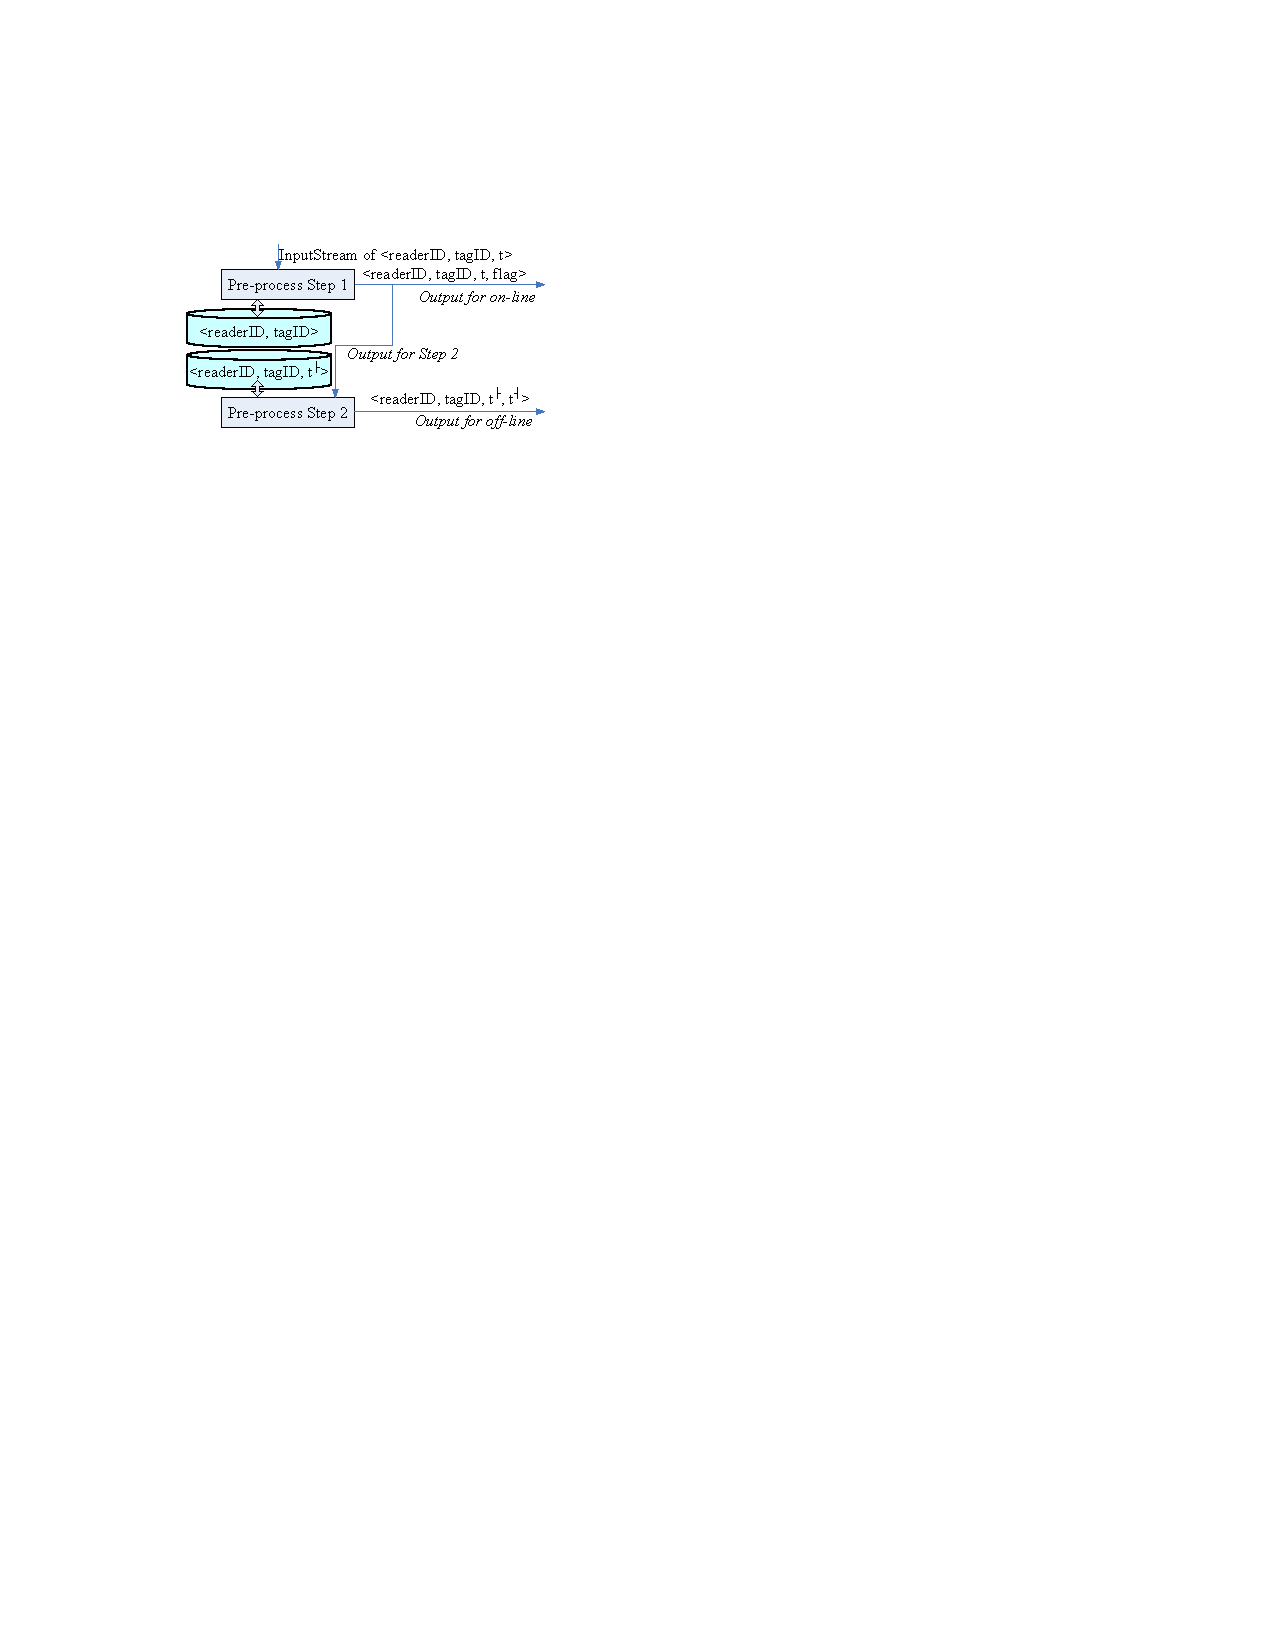
\includegraphics[width=\columnwidth]{figures/2-1-8.pdf}
    \end{figure}

  \column{.53\textwidth}
    \begin{itemize}
        \item $\mathnormal{Flag \in \{ START, END \}}$
        \item $\mathnormal{START} \rightarrow$ \textrm{enters the range}
        \item $\mathnormal{END} \rightarrow$ \textrm{leaves the range}
    \end{itemize}

  \end{columns}

\end{frame}

%------------------------------------------------

\begin{frame}
\frametitle{Off-line Tracking (Refinement Step 1)}

  \begin{columns}[c]

  \column{.43\textwidth}
    \vspace{-15pt}
    \begin{figure}[tb]
      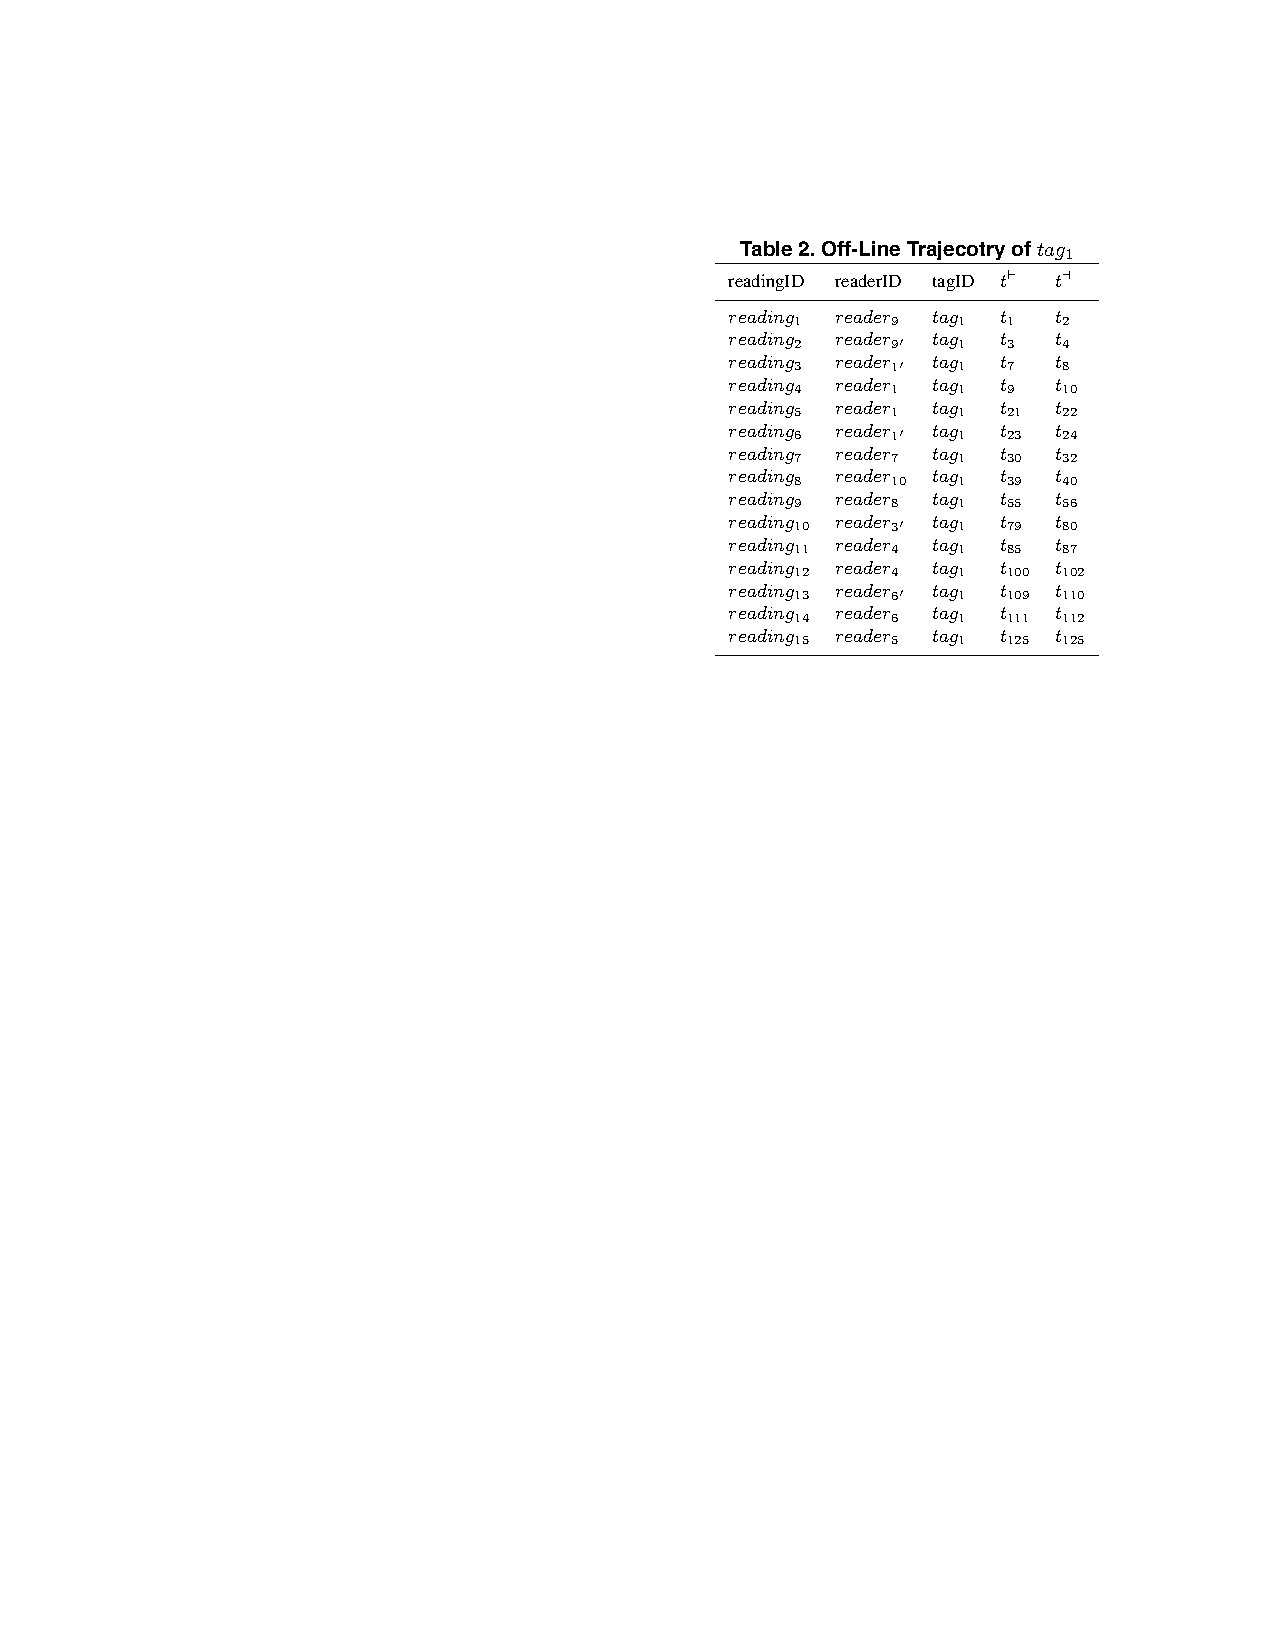
\includegraphics[width=0.92\columnwidth]{figures/2-1-9.pdf}
    \end{figure}
    \vspace{-20pt}
    \begin{figure}[tb]
      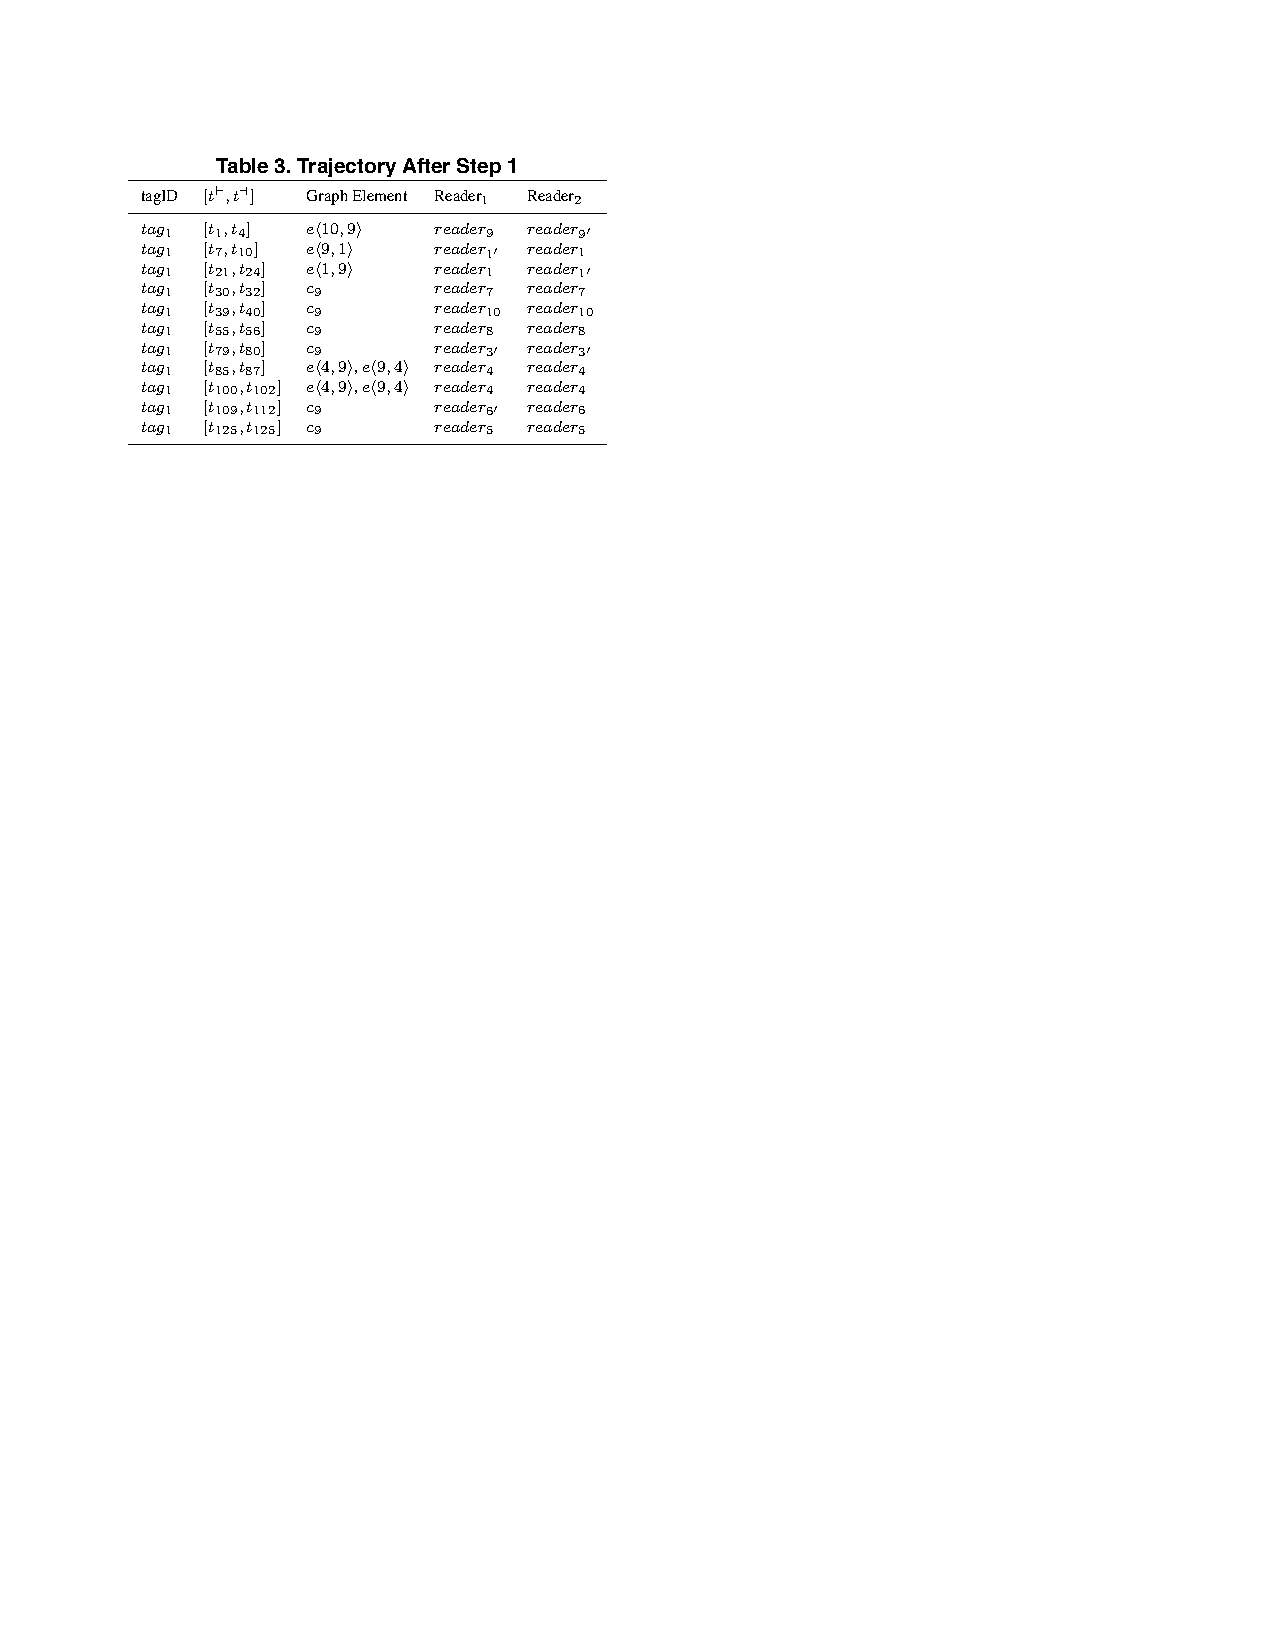
\includegraphics[width=\columnwidth]{figures/2-1-10.pdf}
    \end{figure}


  \column{.57\textwidth}
  \footnotesize{
    \begin{itemize}
      \item Step 1 transforms an RFID reading sequence to corresponding vertices or edges in deployment graph
      \item If two consecutive reading sequences are \emph{contiguous}, they should stem from a partitioning pair, which map to an edge
      \item Otherwise, should come from either a single $\mathnormal{PRE}$ or a $\mathnormal{PAR}$ reader
      \item A $\mathnormal{PAR}$ is replaced by the set of corresponding edges according to $\mathnormal{G_{RFID}.{l_e}^{-1}}$
      \item A $\mathnormal{PRE}$ always coresponds to one or several cells according to $\mathnormal{Mapping~2}$
    \end{itemize}
  }
  \end{columns}

\end{frame}

%------------------------------------------------

\begin{frame}
\frametitle{Off-line Tracking (Refinement Step 2)}

\begin{columns}[c]

  \column{.43\textwidth}
  \vspace{-15pt}
  \begin{figure}[tb]
    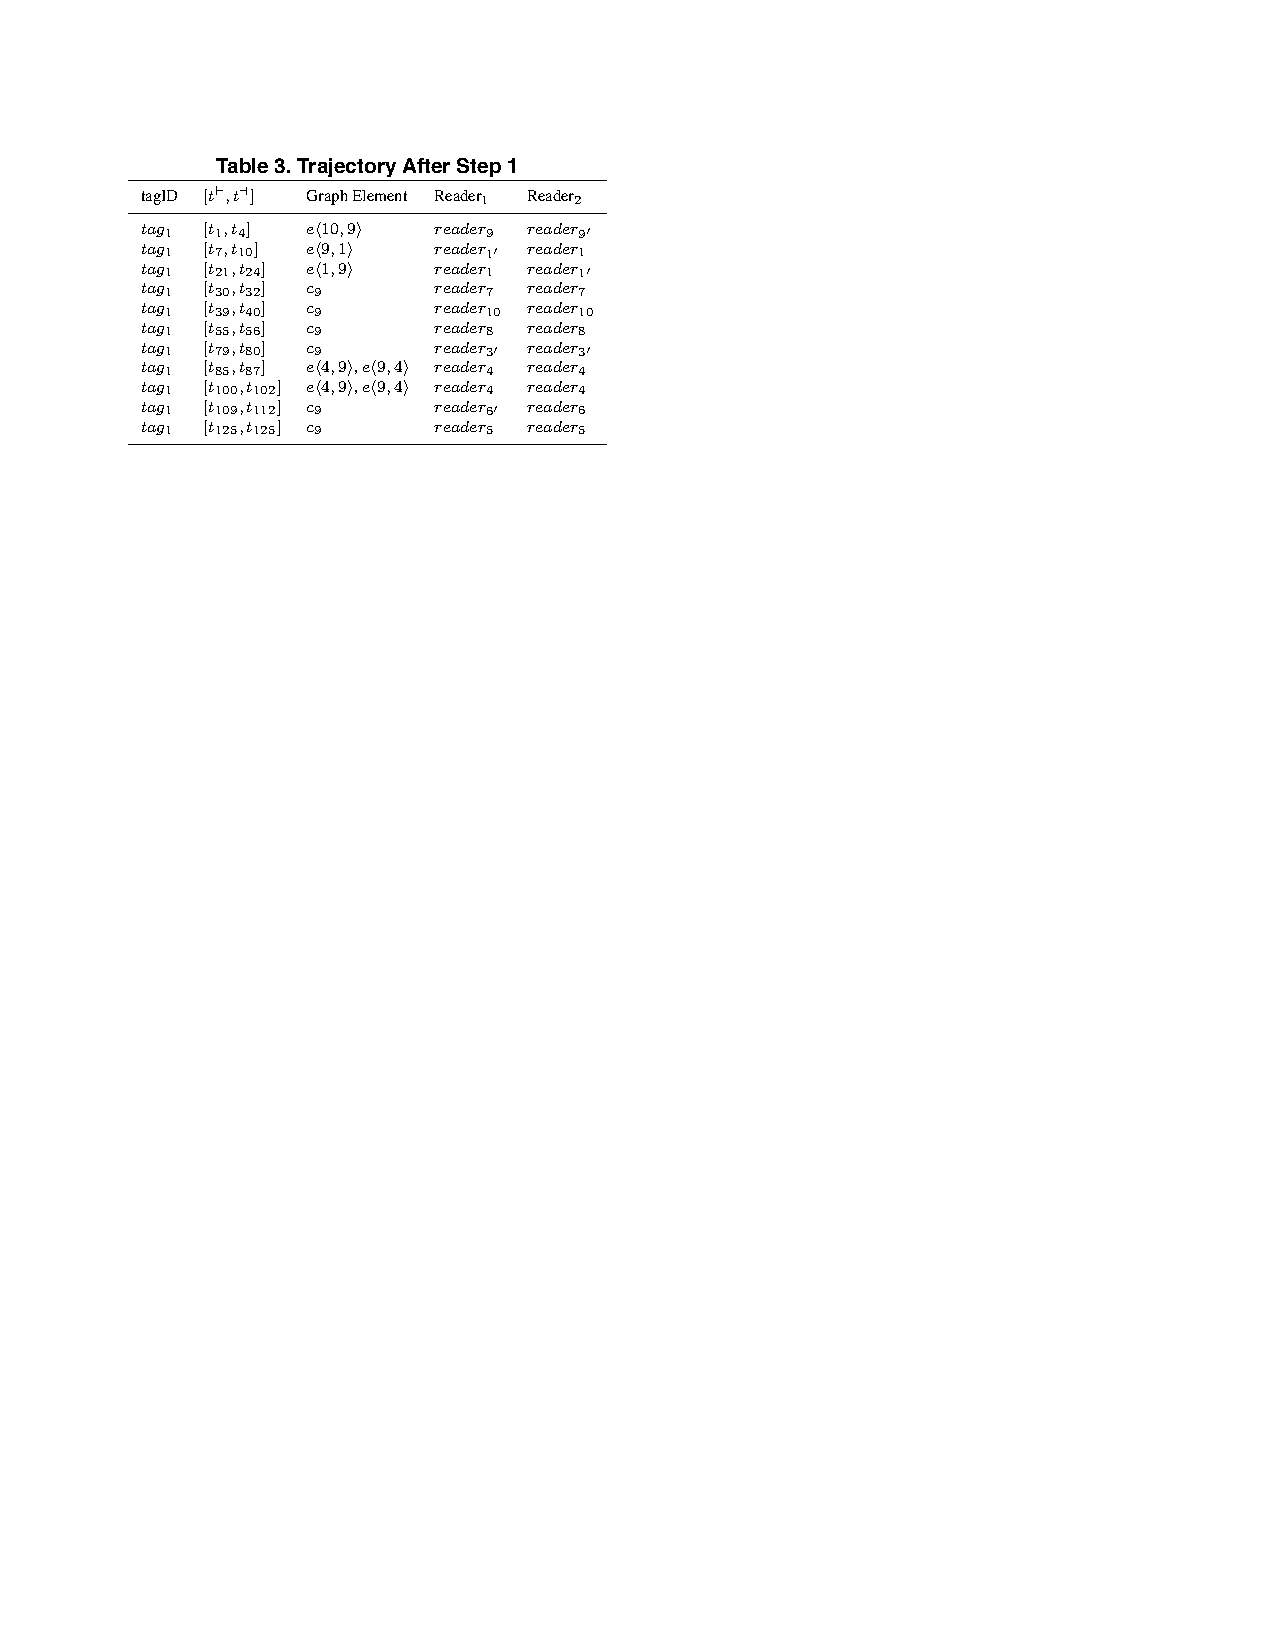
\includegraphics[width=\columnwidth]{figures/2-1-10.pdf}
  \end{figure}
  \vspace{-20pt}
  \begin{figure}[tb]
    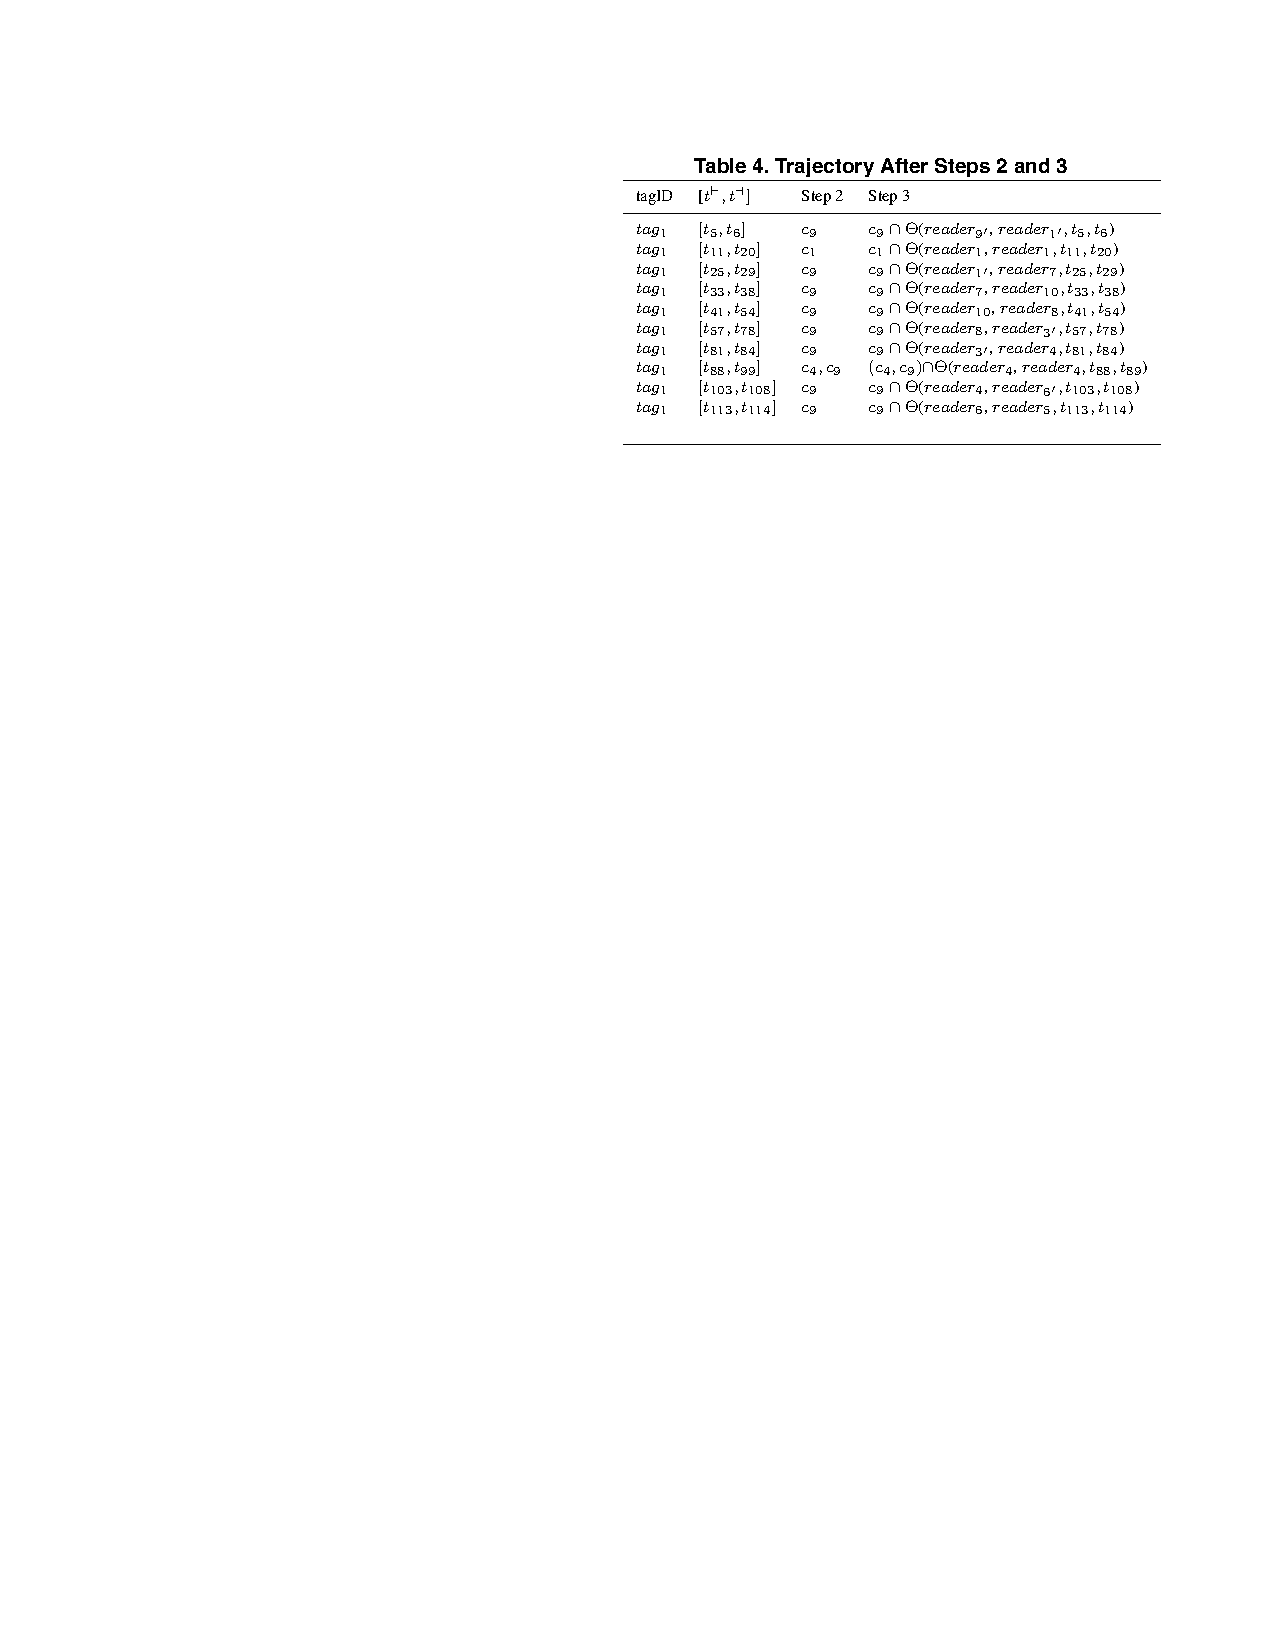
\includegraphics[width=\columnwidth]{figures/2-1-11.pdf}
  \end{figure}


  \column{.57\textwidth}
  \footnotesize{
    \begin{itemize}
      \item The \emph{graph elements} from Step 1 indicates some region(s) within which the object may be in during the vacant time interval
      \item Check its previous record's tail element and current record's head element, select their intersection as Step 2's candidate
    \end{itemize}
  }

\end{columns}

\end{frame}

%------------------------------------------------

\begin{frame}
\frametitle{Off-line Tracking (Refinement Step 3)}

\begin{columns}[c]

\column{.48\textwidth}
\begin{itemize}
\scriptsize{
  \item Calculate the \emph{possible region} $\mathnormal{\Theta}$ according to maximum speed limit

  \item Circle based possible region
    \begin{itemize}
      \tiny{
        \item locations: $\mathnormal{P_{9'}}$, $\mathnormal{P_{1'}}$
        \item activation ranges: $\mathnormal{R_{9'}}$, $\mathnormal{R_{1'}}$
        \item for $\mathnormal{t_x \in [ t_5, t_6 ]}$, $\mathnormal{\Delta t_1 = t_x - reading_2.t^{\vdash}}$, $\mathnormal{\Delta t_2 = reading_3.t^{\dashv} - t_x}$
        \item $\mathnormal{R_3 = R_{9'} + V_{max} * \Delta t_1}$, $\mathnormal{R_5 = R_{1'} + V_{max} * \Delta t_2}$
      }
    \end{itemize}

  \item Ellipse based possible region
  \begin{itemize}
      \tiny{
        \item foci: two points belonging to the circle centered at $\mathnormal{P_{9'}}$, $\mathnormal{P_{1'}}$
        \item length of major axis is:
          \begin{equation*}
            \mathnormal{2a = V_{max} * (\Delta t_1 + \Delta t_2)}
          \end{equation*}
      }
  \end{itemize}
}
\end{itemize}

\column{.52\textwidth}
\vspace{-15pt}
\begin{figure}[tb]
  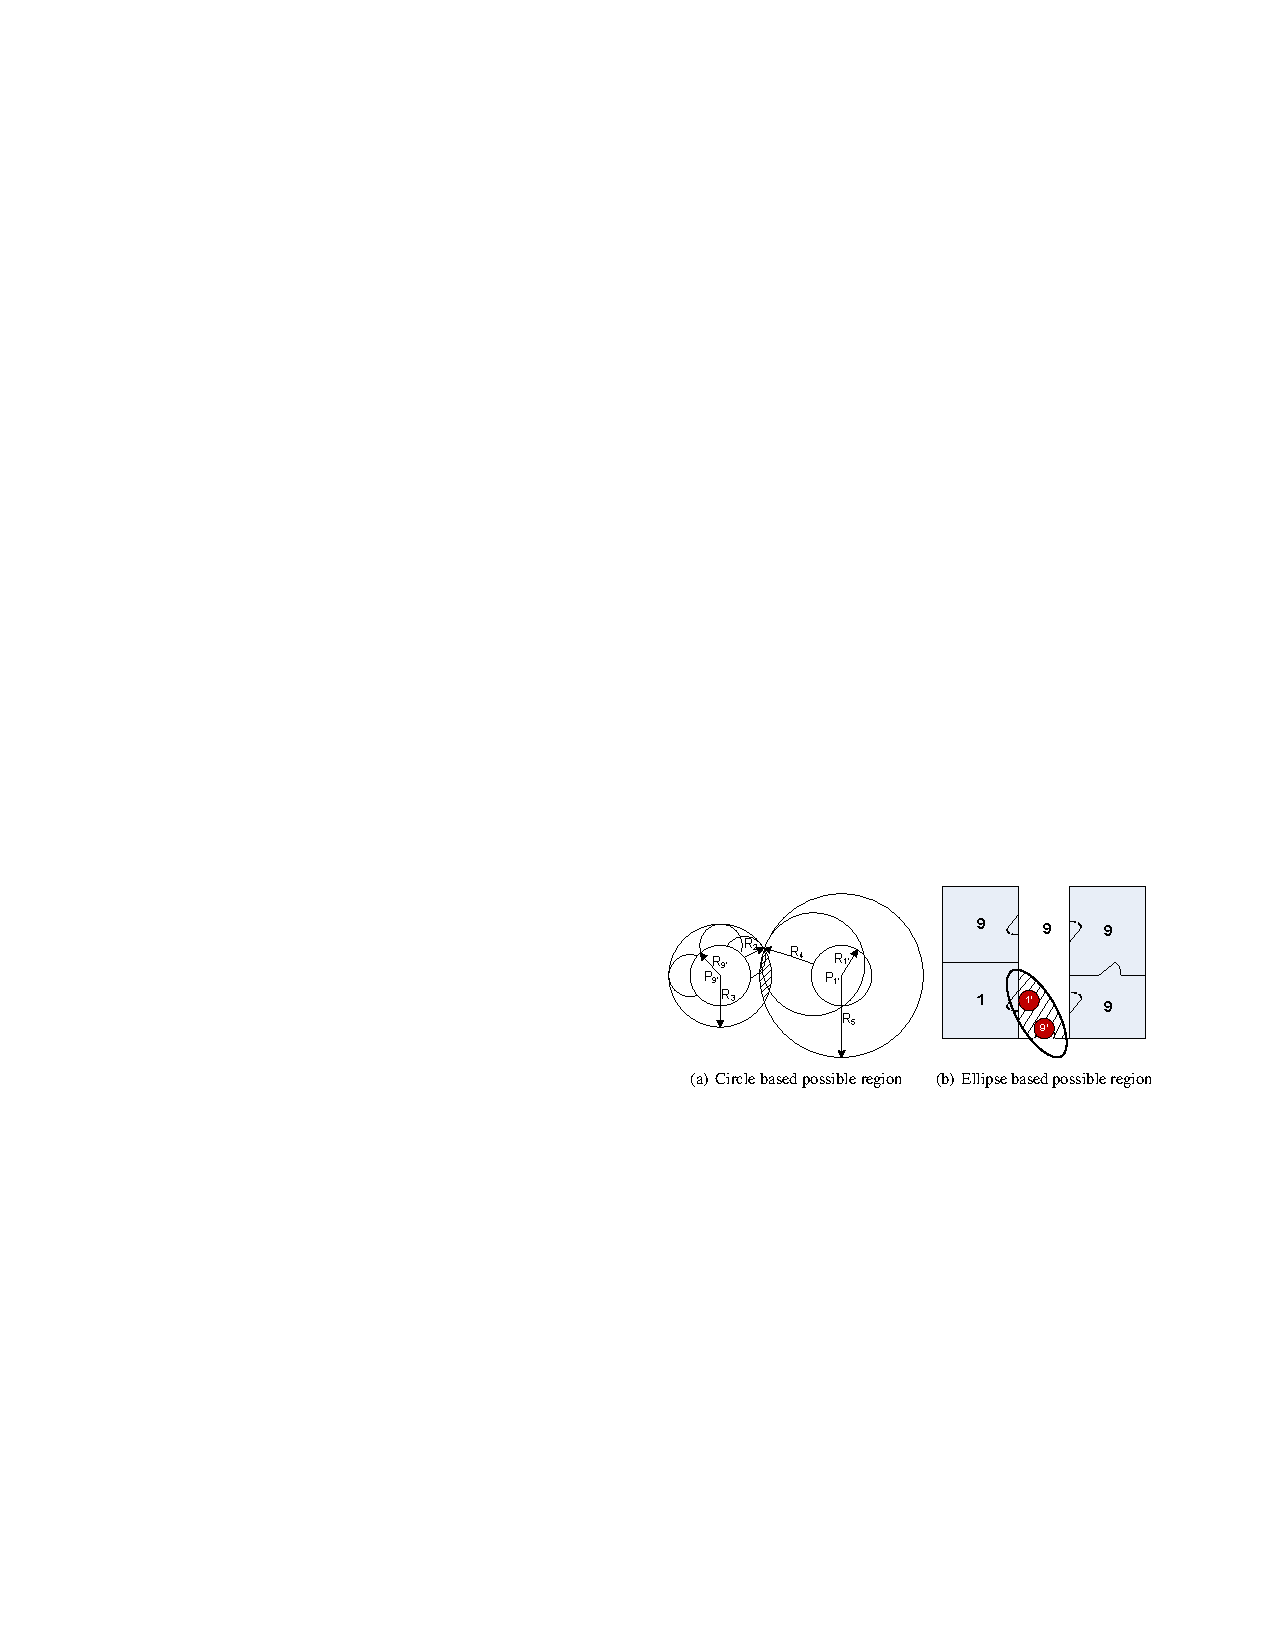
\includegraphics[width=\columnwidth]{figures/2-1-12.pdf}
\end{figure}
\tiny{
  $\left.\begin{matrix}
  \mathnormal{(reading_1, reader_{9}, tag_1, t_1, t_2)}~~\\
  \mathnormal{(reading_2, reader_{9'}, tag_1, t_3, t_4)}~~\\
  \mathnormal{(reading_3, reader_{1'}, tag_1, t_7, t_8)}~~\\
  \mathnormal{(reading_4, reader_{1}, tag_1, t_9, t_10)}~~
  \end{matrix}\right\} \overset{Step~1}{\rightarrow} \pause$ \\~\\~\\

  $\left.\begin{matrix}
  \mathnormal{(tag_1, [t_1,t_4], e\langle 10,9 \rangle, reader_{9}, reader_{9'})}~~\\
  \mathnormal{(tag_1, [t_7,t_{10}], e\langle 9,1 \rangle, reader_{1'}, reader_{1})}~~
  \end{matrix}\right\} \overset{Step~2}{\rightarrow} \pause$ \\~\\~\\

  $\mathnormal{(tag_1, [t_5,t_6], c_9, reader_{9'}, reader_{1'})} \overset{Step~3}{\rightarrow} \pause$ \\~\\~\\

  $\mathnormal{(tag_1, [t_5,t_6], c_9 \cup \Theta(reader_{9'}, reader_{1'}, t_5, t_6))}$
}

\end{columns}

\end{frame}
